\documentclass{standalone}
\usepackage{amsmath,amssymb}
\usepackage{newtxtext,newtxmath}
\usepackage{xcolor}
\usepackage{tikz}
\usetikzlibrary{arrows.meta,positioning,calc,decorations.pathreplacing}

\definecolor{ink}{HTML}{1B1F23}
\definecolor{slate}{HTML}{555E68}
\definecolor{muted}{HTML}{8E96A0}
\definecolor{light}{HTML}{C6CCD2}
\definecolor{faint}{HTML}{E6E9ED}
\definecolor{quantum}{HTML}{2C5E8A}
\definecolor{quantumlight}{HTML}{6C9AC3}
\definecolor{quantumpale}{HTML}{DCE7F2}
\definecolor{ochre}{HTML}{B86B19}
\definecolor{ochrelight}{HTML}{E2B98B}
\definecolor{ochrepale}{HTML}{F6E9D8}

\newcommand{\pfmain}[1]{{\fontsize{7.6}{8.8}\selectfont\color{ink}#1}}
\newcommand{\pfsub}[1]{{\fontsize{7.0}{8.2}\selectfont\color{ink}#1}}
\newcommand{\pfslate}[1]{{\fontsize{7.0}{8.2}\selectfont\color{slate}#1}}
\newcommand{\pfquantum}[1]{{\fontsize{7.0}{8.2}\selectfont\color{quantum}#1}}
\newcommand{\pfochre}[1]{{\fontsize{7.0}{8.2}\selectfont\color{ochre}#1}}

\newcommand{\haty}{%
  \tikz[baseline=(Y.base)]{%
    \node[inner sep=0pt, outer sep=0pt] (Y) {$y$};
    \draw[line width=0.45pt, line cap=round, line join=round]
      ([xshift=0.3pt,yshift=1.25pt]Y.north west) -- ([yshift=2.45pt]Y.north) -- ([xshift=-0.3pt,yshift=1.25pt]Y.north east);
  }%
}

\tikzset{
  pfarrow/.style={-{Stealth[length=3.3pt, width=2.4pt]}, line width=0.65pt, draw=ink},
  pfmutedarrow/.style={-{Stealth[length=3.2pt, width=2.3pt]}, line width=0.60pt, draw=slate},
  pfqgate/.style={
    rectangle, draw=ink, fill=white, line width=0.65pt,
    minimum height=0.225in, inner sep=2.2pt,
    font=\fontsize{7.0}{8.0}\selectfont, text=ink
  }
}


\newcommand{\cnottgt}[2]{%
  \fill[white] (#1,#2) circle[radius=4.0pt];
  \draw[quantum, line width=0.80pt] (#1,#2) circle[radius=4.0pt];
  \draw[quantum, line width=0.80pt] (#1,#2) ++(-4.0pt,0) -- ++(8.0pt,0);
  \draw[quantum, line width=0.80pt] (#1,#2) ++(0,-4.0pt) -- ++(0,8.0pt);
}
\newcommand{\cnotdot}[2]{\fill[quantum] (#1,#2) circle[radius=2.1pt];}

\begin{document}
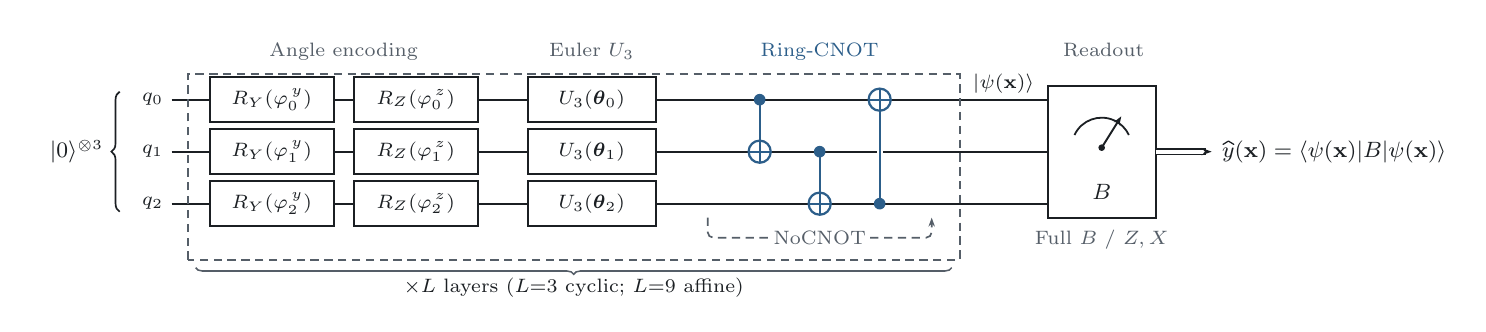
\begin{tikzpicture}[x=1in, y=1in]
  \useasboundingbox (0,-0.12in) rectangle (7.1506in, 1.26in);
  \fill[white] (0,-0.12) rectangle (7.1506, 1.26);

  % Three-qubit data-reuploading ansatz U(x; theta) |0>^{otimes 3} with toggleable ring-CNOT
  \node[anchor=base, inner sep=0pt] at (1.58, 1.115) {\pfslate{Angle encoding}};
  \node[anchor=base, inner sep=0pt] at (2.82, 1.115) {\pfslate{Euler $U_3$}};
  \node[anchor=base, inner sep=0pt] at (3.96, 1.115) {\pfquantum{Ring-CNOT}};
  \node[anchor=base, inner sep=0pt] at (5.38, 1.115) {\pfslate{Readout}};

  \node[anchor=east, inner sep=0pt] at (0.38, 0.64) {\pfmain{$\lvert 0\rangle^{\otimes 3}$}};
  \draw[ink, line width=0.60pt, decorate, decoration={brace, amplitude=3.0pt}]
    (0.46, 0.34) -- (0.46, 0.94);
  \node[anchor=east, inner sep=0pt] at (0.68, 0.90) {\pfsub{$q_0$}};
  \node[anchor=east, inner sep=0pt] at (0.68, 0.64) {\pfsub{$q_1$}};
  \node[anchor=east, inner sep=0pt] at (0.68, 0.38) {\pfsub{$q_2$}};

  \foreach \wy in {0.90, 0.64, 0.38} {
    \draw[ink, line width=0.65pt] (0.72, \wy) -- (5.10, \wy);
  }

  \draw[slate, line width=0.60pt, densely dashed] (0.80, 0.10) rectangle (4.66, 1.03);

  \foreach \q/\wy in {0/0.90, 1/0.64, 2/0.38} {
    \node[pfqgate, minimum width=0.62in] at (1.22, \wy) {$R_Y(\varphi_{\q}^{\,y})$};
    \node[pfqgate, minimum width=0.62in] at (1.94, \wy) {$R_Z(\varphi_{\q}^{\,z})$};
    \node[pfqgate, minimum width=0.64in] at (2.82, \wy) {$U_3(\boldsymbol{\theta}_{\q})$};
  }

  \draw[quantum, line width=0.85pt] (3.66, 0.90) -- (3.66, 0.64);
  \cnotdot{3.66}{0.90}\cnottgt{3.66}{0.64}

  \draw[quantum, line width=0.85pt] (3.96, 0.64) -- (3.96, 0.38);
  \cnotdot{3.96}{0.64}\cnottgt{3.96}{0.38}

  \draw[quantum, line width=0.85pt] (4.26, 0.38) -- (4.26, 0.60);
  \draw[white, line width=2.3pt]    (4.26, 0.61) -- (4.26, 0.67);
  \draw[quantum, line width=0.85pt] (4.26, 0.60) -- (4.26, 0.90);
  \cnotdot{4.26}{0.38}\cnottgt{4.26}{0.90}

  \draw[slate, line width=0.60pt, densely dashed, rounded corners=2pt, -{Stealth[length=3.2pt, width=2.3pt]}]
    (3.40, 0.31) -- (3.40, 0.21) -- (4.52, 0.21) -- (4.52, 0.31);
  \node[anchor=center, fill=white, inner sep=1.2pt] at (3.96, 0.21) {\pfslate{NoCNOT}};

  \draw[slate, line width=0.55pt, decorate, decoration={brace, amplitude=2.4pt, mirror}]
    (0.84, 0.06) -- (4.62, 0.06);
  \node[anchor=north, inner sep=0pt] at (2.73, 0.01)
    {\pfsub{$\times L$ layers ($L{=}3$ cyclic; $L{=}9$ affine)}};

  \node[anchor=south, inner sep=0pt] at (4.88, 0.93) {\pfsub{$\lvert\psi(\mathbf{x})\rangle$}};

  \draw[ink, fill=white, line width=0.70pt] (5.10, 0.31) rectangle (5.64, 0.97);
  \draw[ink, line width=0.65pt] (5.37, 0.66) ++(155:0.15in) arc[start angle=155, end angle=25, radius=0.15in];
  \draw[ink, line width=0.70pt, -{Stealth[length=3.2pt, width=2.3pt]}] (5.37, 0.66) -- ++(58:0.185in);
  \fill[ink] (5.37, 0.66) circle[radius=1.2pt];
  \node[anchor=center, inner sep=0pt] at (5.37, 0.44) {\pfmain{$B$}};
  \node[anchor=north, inner sep=0pt] at (5.37, 0.25) {\pfslate{Full $B$ / $Z,X$}};

  \draw[ink, line width=0.55pt, double, double distance=1.5pt, -{Stealth[length=3.6pt, width=2.6pt]}]
    (5.64, 0.64) -- (5.92, 0.64);
  \node[anchor=west, inner sep=0pt] at (5.97, 0.64)
    {\pfmain{$\haty(\mathbf{x}) = \langle\psi(\mathbf{x})\vert B\vert\psi(\mathbf{x})\rangle$}};
\end{tikzpicture}
\end{document}
